\documentclass[letterpaper, 10 pt, conference]{ieeeconf}

\IEEEoverridecommandlockouts\overrideIEEEmargins
% See the \addtolength command later in the file to balance the column lengths
% on the last page of the document

% The following packages can be found on http://www.ctan.org
\usepackage{graphicx} % for pdf, bitmapped graphics files
%\usepackage{epsfig} % for postscript graphics files
%\usepackage{mathptmx} % assumes new font selection scheme installed
%\usepackage{times} % assumes new font selection scheme installed
\usepackage{amsmath} % assumes amsmath package installed
%\usepackage{amssymb}  % assumes amsmath package installed
\usepackage{url}

\title{\LARGE \bf
Noise Filtering
}

\author{Adari Harshit}

\begin{document}

\maketitle\thispagestyle{empty}
\pagestyle{empty}

%%%%%%%%%%%%%%%%%%%%%%%%%%%%%%%%%%%%%%%%%%%%%%%%%%%%%%%%%%%%%%%%%%%%%%%%%%%%%%%%
\begin{abstract}

Image noise is a common problem in computer vision systems and can reduce the quality of visual information. 
The goal of this project was to explore different image filtering techniques and 
study how noise can be reduced while preserving important features such as edges and structures.

A noise filtering pipeline was implemented using Python and OpenCV to process two corrupted images. 
The work mainly focused on understanding how different filters behave and 
how parameter tuning affects the balance between noise removal and feature preservation. 
The quality of the processed images was evaluated using Signal-to-Noise Ratio (SNR) along with visual inspection.

While working on this task, several core image processing concepts were learned and implemented, 
including grayscale conversion, median filtering, and morphological operations. 
Most of the OpenCV concepts used in this project were learned from the official OpenCV documentation and the FreeCodeCamp OpenCV tutorial.

Noise filtering is an important preprocessing step in aerial robotics systems such as ARK. 
Camera data is used for tasks like line following, object detection, and navigation. 
Reducing noise helps improve the reliability of these perception algorithms and leads to more stable system performance.

\end{abstract}


\section{INTRODUCTION}

Images captured in real world systems often contain noise due to sensor limitations or environmental disturbances. 
This noise can affect the performance because important features such as edges and shapes may become difficult to detect. 
Therefore, noise filtering is an important preprocessing step in many perception pipelines.

The goal of this task was to restore two corrupted images while preserving their important visual structures. 
The first image contains a line drawing of Iron Man corrupted with salt noise. 
The second image contains a natural scenery image corrupted with high-frequency color noise. 
The challenge was to reduce noise while avoiding excessive smoothing that could damage the original features.

To approach this problem, several filtering techniques were tested using OpenCV in Python. 
The process started with basic preprocessing steps such as loading the image and converting it to grayscale where necessary. 
Median filtering was then explored as the primary noise reduction technique because 
it is known to remove noise effectively while preserving edges better than many linear filters.

Morphological image processing techniques were also explored during experimentation. 
Operations such as closing and opening were tested to improve edge continuity and remove small artifacts. 
However, opening operations removed useful edge structures in the Iron Man image, so this approach was discarded. 
Morphological operations were also tested on the natural scenery image but did not significantly improve the results, so they were removed from that pipeline.

Through multiple experiments with different kernel sizes and processing combinations, a balanced approach was developed that reduced noise while maintaining the structural details of the images.


\section{PROBLEM STATEMENT}

The objective of this task is to remove noise from two corrupted images while preserving their important visual features. 
The images provided include a line drawing image corrupted with impulse noise and a natural scenery image corrupted with high-frequency color noise.

Figure \ref{fig:ironman_noisy} shows the Iron Man image affected by salt noise. This type of noise appears as random white pixels scattered across the image. 
Since the image mainly consists of thin edges, aggressive filtering may remove the noise but also damage the line structure.

\begin{figure}[h]
\centering

\includegraphics[width=0.9\columnwidth]{data/iron_man_noisy.jpg}
\caption{Iron Man image corrupted with salt noise}
\label{fig:ironman_noisy}
\end{figure}

Figure \ref{fig:nature_noisy} shows the second corrupted image. In this case the noise appears as random high-frequency variations across the color channels. 
The challenge here is different because the goal is to reduce noise while preserving the natural color structure of the scene.

\begin{figure}[h]
\centering
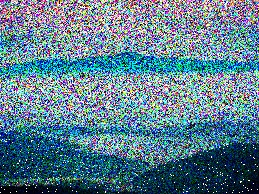
\includegraphics[width=0.9\columnwidth]{data/nature_noisy.jpg}
\caption{Natural scenery image corrupted with high-frequency noise}
\label{fig:nature_noisy}
\end{figure}

To evaluate the effectiveness of the filtering algorithm, Signal-to-Noise Ratio (SNR) was used as a quantitative metric. 
SNR compares the strength of the useful signal to the noise present in the image. It is defined as

\begin{equation}
SNR = 10 \log_{10} \left(\frac{P_{signal}}{P_{noise}}\right)
\end{equation}

where $P_{signal}$ represents the signal power and $P_{noise}$ represents the noise power.

In the implementation, the signal power was computed from the filtered image while the noise was estimated as the difference between the noisy image and the filtered image. 
This gives

\begin{equation}
P_{signal} = \frac{1}{N} \sum_{i=1}^{N} (I_{filtered}(i))^2
\end{equation}

\begin{equation}
P_{noise} = \frac{1}{N} \sum_{i=1}^{N} (I_{noisy}(i) - I_{filtered}(i))^2
\end{equation}

However, in many real-world situations the original clean image is not available. 
For this reason a blind SNR estimation method was also implemented. In this approach, the signal power is estimated using the variance of the image, 
while the noise power is estimated using the variance of the Laplacian operator which highlights high-frequency components such as noise.

\begin{equation}
SNR_{blind} = 10 \log_{10} \left(\frac{\sigma^2(I)}{\sigma^2(\nabla^2 I)}\right)
\end{equation}

where $\sigma^2(I)$ represents the variance of the image and $\sigma^2(\nabla^2 I)$ represents the variance of the Laplacian filtered image.

These metrics help measure how effectively noise is reduced while maintaining the useful structure of the image.


\section{RELATED WORK}

Several filtering techniques have been proposed to remove noise while preserving important image structures. 
The simplest approaches use linear filters such as Gaussian blur to smooth the image and suppress high-frequency noise. 
However, linear filters often blur edges and fine structures, which makes them unsuitable for images that contain thin line features.

Non-linear filters such as the median filter are commonly used to handle impulse noise. 
Unlike linear smoothing filters, the median filter replaces each pixel value with the median value within a local neighborhood. 
This allows it to remove isolated noise pixels while preserving edge boundaries. 
Because of this property, median filtering is widely used for salt-and-pepper noise removal in many applications.

Morphological image processing techniques are also frequently used to improve image quality after filtering. 
Operations such as erosion, dilation, opening, and closing can remove small artifacts and repair broken edges in binary or grayscale images. 
These operations are particularly useful when dealing with line structures or segmented shapes.

During the development of this project, several core image processing concepts were studied and implemented using OpenCV. 
These included image handling operations such as scaling, rotation, and geometric transformations, as well as intensity transformations, image blurring techniques, and feature-related operations such as image alignment. 
These concepts were learned primarily from the official OpenCV documentation and geeksforgeeks.

Understanding these fundamental techniques helped guide the selection of filtering methods and parameter tuning for the noise reduction pipeline implemented in this project.


\section{INITIAL ATTEMPTS}

The first step was to study the type of noise present in both images. The Iron Man image contained salt noise. This appeared as random white pixels across the drawing. 
The nature image contained high-frequency noise spread across the color channels.

The first experiments used median filtering with different kernel sizes. A kernel size of 1 was tested initially. 
This produced almost no change in the image because the filter behaved like an identity operation. 
As a result, most of the noise remained in the output.

A larger kernel size of 5 was also tested. This removed many noise pixels but caused noticeable distortion in the thin line structures of the Iron Man image. 
Important edges became thicker or partially blurred. This made the drawing lose some of its structural detail.

Morphological operations were also tested during early experiments. Opening was applied after median filtering to remove isolated pixels. 
However, this operation removed some useful edge pixels from the Iron Man drawing. As a result, parts of the line structure were broken. 
Because of this issue, the opening operation was removed from the final pipeline.

Morphological processing was also tested for the nature image. The goal was to remove remaining noise artifacts after filtering. 
However, the results did not improve the image significantly. In some cases the image structure was slightly distorted. 
Therefore morphology was not used for the nature image.

Through these experiments it became clear that careful parameter tuning was required. 
The final approach was chosen based on both visual inspection and Signal-to-Noise Ratio evaluation.


\section{FINAL APPROACH}

After multiple experiments, a noise filtering pipeline was designed to remove noise while preserving important image structures. 
The final solution was implemented using OpenCV in Python. The pipeline contains three main stages: preprocessing, filtering, and evaluation.

\subsection{Image Preprocessing}

The first step is loading the corrupted image using OpenCV. For the Iron Man image, the image is converted to grayscale before filtering. 
Since the image mainly contains line structures, grayscale processing simplifies the filtering operation while preserving the shape information.

For the natural scenery image, the filtering is applied directly on the color image. This preserves the color structure of the scene while reducing high-frequency noise.

\subsection{Median Filtering}

Median filtering is used as the primary noise removal technique. 
Unlike linear filters, the median filter replaces each pixel value with the median value from its neighborhood. This makes it highly effective for removing impulse noise.

Mathematically, the median filtering operation can be written as

\begin{equation}
I_{out}(x,y) = \text{median}\{I(i,j)\}
\end{equation}

where $(i,j)$ represents the neighborhood around the pixel $(x,y)$.

Median filtering removes isolated noisy pixels while preserving sharp edges. 
This property makes it suitable for restoring the Iron Man line drawing.

\subsection{Morphological Processing}

Morphological closing was applied to the Iron Man image after median filtering. 
This operation helps reconnect small gaps that appear in thin line structures after noise removal.

The closing operation is defined as

\begin{equation}
A \bullet B = (A \oplus B) \ominus B
\end{equation}

where $\oplus$ represents dilation and $\ominus$ represents erosion.

This step improves the continuity of edges in the drawing without introducing additional smoothing.

Morphological operations were not applied to the natural scenery image because they did not noticeably improve the visual quality during experimentation.

\subsection{Parameter Selection}

Different kernel sizes were tested during experimentation. The final parameters were selected based on a balance between noise removal and feature preservation.

For the Iron Man image:

\begin{itemize}
\item Median filter kernel size = 3
\item Morphological kernel size = 3
\end{itemize}

For the natural scenery image:

\begin{itemize}
\item Median filter kernel size = 5
\end{itemize}

These parameters provided the best balance between noise suppression and edge preservation.

\subsection{Quality Evaluation}

The performance of the filtering process was evaluated using Signal-to-Noise Ratio (SNR). 
Additionally, a blind SNR estimate was computed using the variance of the Laplacian operator.

These metrics help quantify how effectively noise is reduced while maintaining useful image information.


\section{RESULTS AND OBSERVATIONS}

The proposed filtering pipeline was tested on the two corrupted images provided in the task. 
The effectiveness of the algorithm was evaluated using both visual inspection and Signal-to-Noise Ratio (SNR) measurements.

\subsection{Iron Man Image}

Figure \ref{fig:ironman_result} shows the output obtained after applying median filtering and morphological processing to the corrupted Iron Man image.

\begin{figure}[h]
\centering
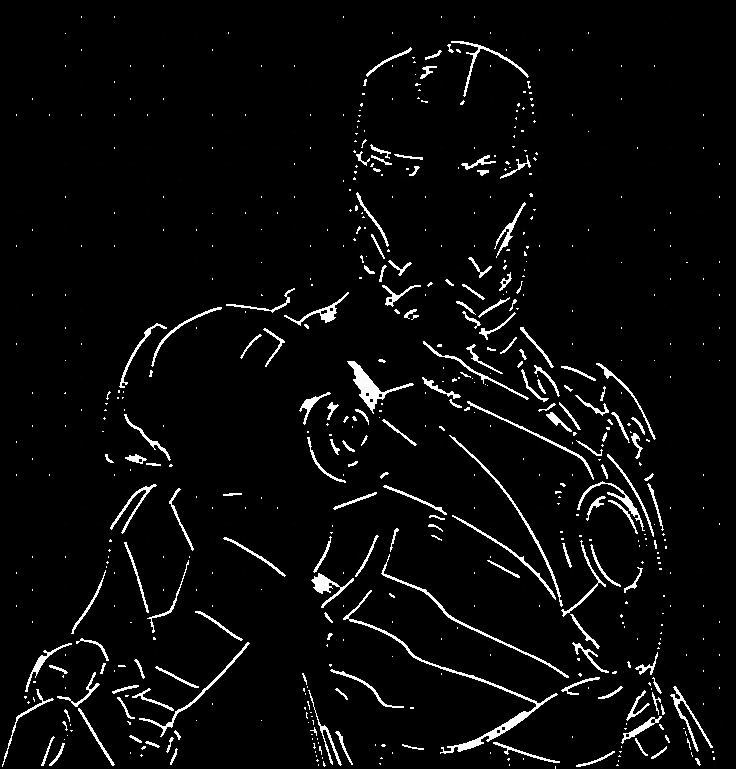
\includegraphics[width=0.9\columnwidth]{output/iron_man_denoised.jpg}
\caption{Filtered Iron Man image after noise removal}
\label{fig:ironman_result}
\end{figure}

The median filter successfully removed a large portion of the salt noise while preserving the thin edge structures of the drawing. 
The morphological closing operation helped reconnect small gaps in the line structures that appeared during filtering.

The final Signal-to-Noise Ratio obtained for the Iron Man image was:

\begin{center}
SNR = 4.92 dB
\end{center}

Although higher kernel sizes removed more noise visually, they also damaged the original line structure. 
The chosen parameters therefore provided a better balance between noise removal and feature preservation.

\subsection{Natural Scenery Image}

Figure \ref{fig:nature_result} shows the result obtained for the natural scenery image after applying median filtering.

\begin{figure}[h]
\centering
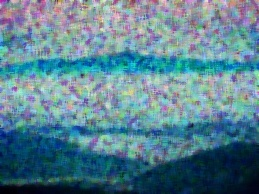
\includegraphics[width=0.9\columnwidth]{output/nature_denoised.jpg}
\caption{Filtered natural scenery image}
\label{fig:nature_result}
\end{figure}

The median filter reduced a large portion of the high-frequency noise while maintaining the overall color structure of the image. 
Unlike the Iron Man image, morphological operations were not applied because they did not significantly improve the result during experimentation.

The final Signal-to-Noise Ratio obtained for the nature image was:

\begin{center}
SNR = 6.82 dB
\end{center}

\subsection{Observations}

Several important observations were made during the experiments:

\begin{itemize}

\item Small median kernels preserve edges but remove less noise.

\item Large kernels remove more noise but may blur important image features.

\item Morphological operations are effective for line-based images but are less useful for natural scene images.

\item A balance between visual quality and numerical metrics such as SNR is necessary for effective denoising.

\end{itemize}


\section{FUTURE WORK}

Although the implemented filtering pipeline produced good results, several improvements can be explored in future work.

One limitation of the current evaluation is the absence of a clean reference image. 
If a ground truth image were available, more accurate metrics such as Peak Signal-to-Noise Ratio (PSNR) could be used to measure restoration quality more reliably.

The current filtering method uses fixed kernel sizes. In future work, adaptive filtering techniques could be explored where the filter size changes based on the noise level or local image features.

More advanced denoising algorithms could also be investigated. 

Another possible improvement is automatic parameter tuning. Instead of manually selecting kernel sizes, optimization methods could be used to select parameters that maximize image quality metrics.

These improvements could lead to more robust noise removal systems that perform better across different types of images and noise conditions.



\section*{CONCLUSION}


This project focused on restoring corrupted images affected by different types of noise using image processing techniques. 


A noise filtering approach was implemented using Python and OpenCV. Median filtering was used as the primary denoising method due to its ability to remove impulse noise while maintaining edge structures. 

Morphological processing was applied selectively to improve the continuity of line structures in the Iron Man image. 


The results showed that parameter tuning plays a critical role in image denoising. Aggressive filtering can remove noise but may also destroy important details, while insufficient filtering leaves noise artifacts in the image. 

Therefore, achieving the right balance between noise removal and feature preservation is essential.


Noise filtering is an important preprocessing step in aerial robotics systems such as ARK. Vision-based tasks rely on clean visual input. 

Improving image quality before further processing helps increase the reliability and stability of these perception algorithms.


Overall, this work demonstrates how fundamental computer vision techniques can be used to design effective noise reduction pipelines for real-world perception tasks.



\begin{thebibliography}{99}


\bibitem{c1}
GeeksforGeeks, ``OpenCV Python Tutorial,'' Available:
\url{https://www.geeksforgeeks.org/python/opencv-python-tutorial/}

\bibitem{c2}
OpenCV Documentation, ``OpenCV Python Tutorials,'' Available:
\url{https://docs.opencv.org/3.0-beta/doc/py_tutorials/py_tutorials.html}

\bibitem{c3}
FreeCodeCamp, ``OpenCV Course – Full Computer Vision Tutorial,'' YouTube Video. Available:
\url{https://www.youtube.com/watch?v=P4Z8_qe2Cu0}

\bibitem{c4}
Kevin Wood Robotics, ``Computer Vision and Robotics Tutorials,'' YouTube Channel. Available:
\url{https://www.youtube.com/@kevinwoodrobotics}


\end{thebibliography}


\end{document} 
